\documentclass[11pt,twocolumn]{article}

\usepackage[includehead,margin=0.5in]{geometry}
\usepackage{fancyhdr}
\usepackage{amsmath}
\usepackage{graphicx}
\usepackage{helvet}
\renewcommand{\familydefault}{\sfdefault}

\title{\textbf{
  FAST SYMBOLIC METHODS FOR MUSCLE-DRIVEN\\
  OPTIMAL CONTROL AND PARAMETER IDENTIFICATION
}}
\author{
Jason K. Moore\textsuperscript{1}\and
Samuel G. Brockie\textsuperscript{2}\and
Timótheüs J. Stienstra\textsuperscript{1}\and
Antonie van den Bogert\textsuperscript{3}\\
\textsuperscript{1}Department of BioMechanical Engineering, Delft University of Technology, The Netherlands\\
Startup, United Kingdom\\
\textsuperscript{3}Mechanical Engineering, Cleveland State University, USA\\
Email: j.k.moore@tudelft.nl}
\date{}


\renewcommand{\thispagestyle}[1]{} % do nothing

\begin{document}
\pagestyle{fancy}
\lhead{}
\rhead{XX International Symposium on Computer Simulation in Biomechanics\\
July 23rd – 25th 2025, Uppsala} %empty
\maketitle
\section*{INTRODUCTION}
%
Direct collocation has grown rapidly for solving biomechanical optimal control
problems. For example, OpenSim now includes Moco~\cite{Dembia2019} which allows
users to find solutions with relatively low user overhead. One advantage of
direct collocation when compared to shooting optimization methods is the speed
at which solutions can be found. The computation costs can be orders of
magnitude faster with direct collocation. But direct collocation methods rely on
local minimization techniques and computational cost can still increase when
searching for global minima.

Direct collocation methods require evaluating the system's equations of motion,
its Jacobian, and possibly its Hessian thousands to millions of times for one
solution, but this evaluation is easily parallelizable over multiple compute
cores and can leverage the massive sparsity of the equations. This cannot be, in
general, done in shooting methods that require sequential integration stepping.
Maximizing the compute and memory performance of the functions that evaluate the
constraints and their derivatives allows the subsequent optimization algorithms
to solve very large problems, both in simulation duration and number of degrees
of freedom.

Early dynamics simulation software used computer-aided algebra techniques, which
allowed for analytical derivatives when forming equations of motion, but this
has faded from popularity with growth of numerical physics engines. Code
generated from computer aided algebra can be optimized for evaluation
performance using compiler pre-optimizations and built-in compiler optimizations
that are harder, or impossible, to apply to numeric physics engines.

We will demonstrate software that leverages symbolic formulations to generate
computationally efficient parallelized functions to evaluate the non-linear
programming problem's constraints and its derivatives. We will show an
arm-muscle driven bicycle-rider model that has XXX million floating point
operations for evaluating the constraints and its Jacobian.

\section*{METHODS}
%
The non-linear equations of motion for musculoskeletal system can be described
by differential algebraic equations that are a function of the state
\(\mathbf{y}\), controls \(\mathbf{r}\), and constant parameters
\(\mathbf{p}\), in general. These equations take this form:
%
\begin{align}
  \mathbf{f}(\dot{\mathbf{y}}(t), \mathbf{y}(t), \mathbf{r}(t), \mathbf{p}) =
  \mathbf{0} \in \mathrm{R}^n
\end{align}
%
These equations can contain elements such as musculotendon force-velocity
relationships, kinematic loops, friction, collision, etc. We write these
equations as analytically differentiable functions. The Jacobian and Hessian can
be formed by recursive symbolic differentiation. To map these to non-linear
programming constraints we discretize the equations with backward Euler
differentiation over a constant time step and code generate functions in C that
evaluate the constraints and Jacobian over all nodes, while exploiting the high
sparsity of the Jacobian~\cite{Moore2018}. The symbolic Jacobian is calculated
in forward mode applying the chain rule through all common sub-expressions which
handles large equations of motion. This results in cacheable computationally
efficient numerical functions that evaluate the non-linear programming problem
constraints and its Jacobian. Evaluation of the objective is generally a low
computational cost, so this is only done in Python, also with a symbolic to
numeric conversion.
%
\begin{table*}[t]
  \centering
  \caption{Mean performance values for the arm-muscle driven bicycle model lane
  change maneuver on a Macbook Pro XXX.}
  \scriptsize
  \begin{tabular}{lllllllllll}
    Symbolic & Symbolic & OCP & Constraint & Jacobian  & Jacobian & NLP & Objective &  Gradient & Constraint & Jacobian \\
    EOM & OCP & Solve & Compilation &  Compilation & Differentiation & iterations & evaluations & evaluations & evaluations & evaluations \\
    14.9 & 169.8 & 73.0 & 58.3 & 66.7 & 35.4 & 286 & 1098 & 286 & 1098 & 292
  \end{tabular}
  \label{tab:performance}
\end{table*}

\section*{RESULTS AND DISCUSSION}
%
To demonstrate the qualities of our methods we have developed a bicycle-rider
model that includes the non-linear Carvallo-Whipple of the vehicle and with four
additional rigid bodies representing the upper and lower arm body
segments~\cite{Stienstra2023a}. The arms are added in such a way that no
additional degrees of freedom are added to the vehicle model due to the
closed-loop kinematic constraints. The model has seven holonomic constraints and
four nonholonomic constraints . We include four lumped Hill-Type muscle models
representing the extensor and flexor groups for the elbow. This results in a set
of differential algebraic equations with 2.8M floating point operations in the
symbolic equations of motion. After compiler pre-optimizations, this reduces to
XK and XM, for the constraints and Jacobian respectively. Once the constraints
and Jacobian NLP numerical evaluation functions are rewritten the evaluation
time depends on the number of nodes. For X nodes we time the evaluation of these
two functions with and without parallelization using from OpenMP. We then solve
the optimal control problem defined by the objective to follow a lane change
path with the front wheel.

\begin{figure}
    \centering
    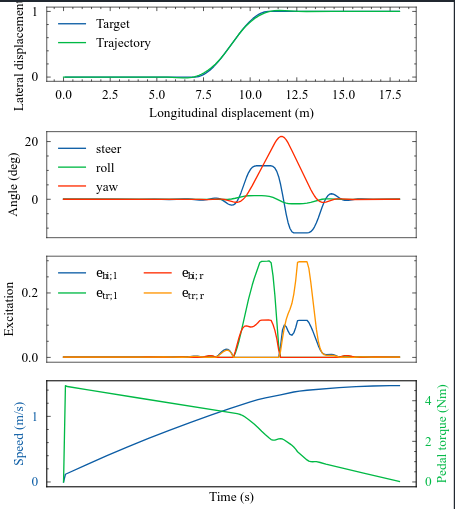
\includegraphics[width=\linewidth]{figures/arm-muscle-bicycle-excitation.png}
    \caption{Triceps and biceps muscle group excitations for the left and right arms to execute a lane change maneuver.}
    \label{fig:enter-label}
\end{figure}

The timings are shown in Table~\ref{tab:performance}. Building the model and
forming the optimal control problem takes 185 seconds with most time spent
compiling the generated functions with Clang. This can be cached to disk and
need not be built again unless the dynamics model changes. IPOPT solves the
problem to an acceptable level in 73 seconds.

\section*{CONCLUSIONS}

\bibliography{references}
\bibliographystyle{plain}

\end{document}
